\documentclass[10pt,a4paper]{article}
\usepackage[margin=21mm,headheight=15pt]{geometry}
\usepackage[T1]{fontenc}
\usepackage{lmodern,amsmath,amssymb,tikz,graphicx,hyperref,fancyhdr,enumitem}
\usetikzlibrary{arrows.meta,positioning,calc,decorations.pathmorphing}
\definecolor{ink}{RGB}{20,53,78}
\hypersetup{colorlinks=true,urlcolor=ink,linkcolor=ink}
\setlength{\parindent}{0pt}\setlength{\parskip}{5pt}
\emergencystretch=3em
\pagestyle{fancy}\fancyhf{}\fancyfoot[C]{\thepage}
\renewcommand{\headrulewidth}{.3pt}
\newcommand{\task}[2]{\par\medskip{\color{ink}\Large\bfseries #1. #2}\par\smallskip}
\newcommand{\answer}{\par\smallskip\textbf{Worked reasoning.} }
\setlist[enumerate]{label=\textbf{(\alph*)},leftmargin=7mm,itemsep=7pt}
\begin{document}
\fancyhead[L]{\small Control of Dynamical Systems}
\fancyhead[R]{\small Laboratory 08}
{\color{ink}\LARGE\bfseries Laboratory 08}\par
{\large Lead-lag design for a normalized camera axis}\par
\textbf{Worked solutions -- five integrated problems}\par
{\small\textbf{Evidence boundary.} Original hypothetical scenarios. Derive, calculate and justify decisions; every numerical record is synthetic. Figures are conceptual and not to scale.}
\smallskip\textbf{Shared nominal data.} Nominal camera-axis plant: $G(s)=1/[s(s+1)]$. Design crossover is 3 rad/s and desired phase margin is $55^\circ$. Use unrounded compensator parameters in subsequent calculations.
\task{1}{A camera axis with simultaneous speed and phase requirements}
The physical sketch shows a single rotating camera axis with a position sensor. The normalized transfer is stipulated; inertia, drive bandwidth and unit scaling are already aggregated into it.
\begin{center}\resizebox{.80\linewidth}{!}{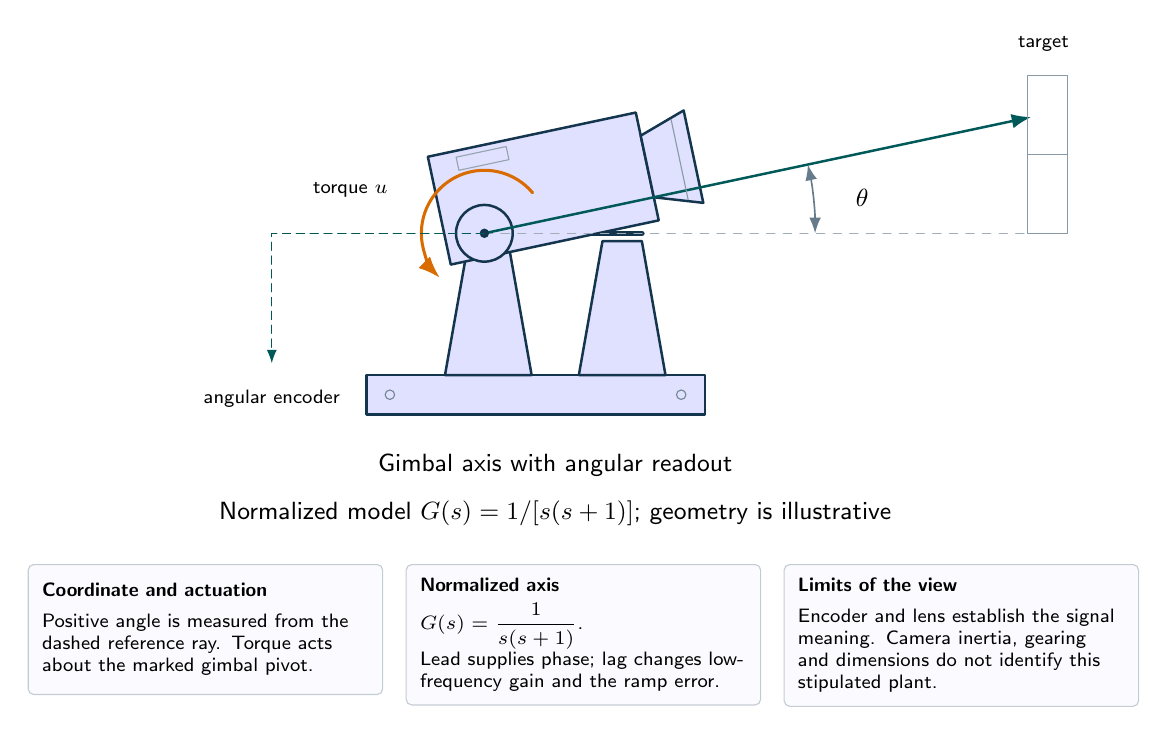
\begin{tikzpicture}[
font=\sffamily\small,>=Latex,line cap=round,line join=round,
wall/.style={draw=ink,line width=1.2pt,fill=blue!5},
water/.style={fill=cyan!25,draw=none},
metal/.style={draw=ink,fill=blue!12,line width=.9pt},
flow/.style={->,draw=blue!65!black,line width=1.2pt},
heat/.style={->,draw=orange!85!black,line width=1.1pt},
measure/.style={->,draw=teal!70!black,line width=.9pt},
dim/.style={<->,draw=ink!65,line width=.6pt},
spring/.style={draw=ink,decorate,decoration={coil,aspect=.5,segment length=4pt,amplitude=3pt}},
wire/.style={draw=ink,line width=1pt},
lab/.style={align=center,font=\sffamily\small},
smalllab/.style={align=center,font=\sffamily\scriptsize}]

\draw[metal](4.3,.4)rectangle(8.6,.9);
\draw[metal](5.3,.9)--(5.6,2.6)--(6.1,2.6)--(6.4,.9)--cycle;
\draw[metal](7,.9)--(7.3,2.6)--(7.8,2.6)--(8.1,.9)--cycle;
\draw[ink,line width=2pt](5.7,2.7)--(7.8,2.7);
\draw[metal,rotate around={12:(5.8,2.7)}](5.3,2.4)rectangle(8,3.8);
\draw[metal,rotate around={12:(5.8,2.7)}](8,2.7)--(8.6,2.5)--(8.6,3.7)--(8,3.5)--cycle;
\draw[metal](5.8,2.7)circle(.36);
\draw[heat]($(5.8,2.7)+(40:.8)$)arc[start angle=40,end angle=225,radius=.8];
\node[smalllab]at(4.1,3.25){torque $u$};
\draw[ink!40,dashed](5.8,2.7)--(12.7,2.7);
\draw[measure](5.8,2.7)--++(12:7.1);
\draw[dim]($(5.8,2.7)+(0:4.2)$)arc[start angle=0,end angle=12,radius=4.2];
\node[lab]at(10.6,3.15){$\theta$};
\draw[ink!50](12.7,2.7)rectangle(13.2,4.7);
\draw[ink!50](12.7,3.7)--(13.2,3.7);
\node[smalllab]at(12.9,5.1){target};
\node[lab]at(6.7,-.25){Gimbal axis with angular readout};
\node[lab]at(6.7,-.85){Normalized model $G(s)=1/[s(s+1)]$; geometry is illustrative};
% REFINED EQUIPMENT DETAILS

% Resolved camera lens, mounting bolts, encoder readout and pivot.
\foreach \x in {4.6,8.3}{\draw[ink!60](\x,.65)circle(.06);}
\draw[ink!50,rotate around={12:(5.8,2.7)}](8.42,2.58)--(8.42,3.62);
\draw[ink!45,rotate around={12:(5.8,2.7)}](5.65,3.55)rectangle(6.3,3.72);
\fill[ink](5.8,2.7)circle(.06);
\draw[teal!70!black,densely dashed,->](5.8,2.7)--(3.1,2.7)--(3.1,1.05);
\node[smalllab]at(3.1,.6){angular encoder};

\node[draw=ink!25,fill=blue!2,rounded corners=2pt,anchor=north west,text width=4.15cm,minimum height=1.65cm,inner sep=5pt,align=left,font=\sffamily\scriptsize]at(0.0,-1.5){\textbf{Coordinate and actuation}\\[3pt]Positive angle is measured from the dashed reference ray. Torque acts about the marked gimbal pivot.};
\node[draw=ink!25,fill=blue!2,rounded corners=2pt,anchor=north west,text width=4.15cm,minimum height=1.65cm,inner sep=5pt,align=left,font=\sffamily\scriptsize]at(4.8,-1.5){\textbf{Normalized axis}\\[3pt]$G(s)=\dfrac{1}{s(s+1)}$.\\Lead supplies phase; lag changes low-frequency gain and the ramp error.};
\node[draw=ink!25,fill=blue!2,rounded corners=2pt,anchor=north west,text width=4.15cm,minimum height=1.65cm,inner sep=5pt,align=left,font=\sffamily\scriptsize]at(9.6,-1.5){\textbf{Limits of the view}\\[3pt]Encoder and lens establish the signal meaning. Camera inertia, gearing and dimensions do not identify this stipulated plant.};
\end{tikzpicture}
}\par{\small A camera gimbal illustrates angular tracking and disturbance rejection. Its normalized plant is stipulated, with no claim that geometry alone determines its two poles.}\end{center}
\begin{enumerate}
\item The normalized plant is $G(s)=1/[s(s+1)]$. At unity controller gain, derive the closed-loop polynomial, gain crossover and phase margin.
\answer The closed polynomial is $s^2+s+1$, so the baseline loop is stable. Magnitude one requires $\omega^2(1+\omega^2)=1$, hence $\omega_c=\sqrt{(\sqrt5-1)/2}$. The phase is $-90^\circ-\arctan\omega_c$ and the phase margin is $90^\circ-\arctan\omega_c\approx51.83^\circ$. These values characterize the baseline before a new crossover is imposed.
\item A redesign targets crossover 3 rad/s and phase margin 55 degrees. Compute the plant phase at that frequency and the phase the lead section must provide. Explain why changing scalar gain alone cannot achieve both targets.
\answer At $\omega=3$, plant phase is $-90^\circ-\arctan3\approx-161.565^\circ$. A 55 degree margin requires loop phase $-125^\circ$, so the controller must provide $\phi=\arctan3-35^\circ\approx36.565^\circ$. A positive scalar gain changes magnitude but not phase at the specified frequency. It can place the crossover at 3, but would leave only about 18.435 degrees of margin.
\item Suppose an omitted actuator lag $1/(0.1s+1)$ is added to the plant. At the fixed 3 rad/s crossover, find the scalar gain needed for unity magnitude, the resulting phase margin, and the lead phase now required for the $55^\circ$ target. Compare with the original plant.
\answer The augmented magnitude is $1/[3\sqrt{10}\sqrt{1+0.3^2}]$, so the scalar gain is $K=3\sqrt{10.9}\approx9.90454$. The lag also subtracts $\tan^{-1}(0.3)\approx16.69924^\circ$. The remaining margin is $90^\circ-\tan^{-1}(3)-\tan^{-1}(0.3)\approx1.73570^\circ$, leaving a required lead of approximately $53.26430^\circ$. The original plant needed only $36.56505^\circ$. Restoring crossover by gain adjustment therefore does not recover the original phase budget; omitted actuator dynamics materially change the compensator design.
\end{enumerate}

\newpage
\task{2}{Realizing and normalizing a lead network}
The desired phase improvement must be produced by a realizable pole--zero pair and then normalized at the selected frequency.
\begin{enumerate}
\item For $C_{lead}=K(Ts+1)/(\alpha Ts+1)$, center maximum phase lead at 3 rad/s and supply the phase found in Problem 1(b). Derive $\alpha$ and T and locate the controller zero and pole.
\answer Use $\sin\phi=(1-\alpha)/(1+\alpha)$, giving $\alpha=(1-\sin\phi)/(1+\sin\phi)$. Centering the phase peak requires $3=1/(T\sqrt\alpha)$, so $T=1/(3\sqrt\alpha)$. The zero is $-1/T=-3\sqrt\alpha$ and the pole is $-1/(\alpha T)=-3/\sqrt\alpha$. Since $0<\alpha<1$, the pole lies farther left than the zero. These positions produce positive phase lead between their break frequencies.
\item Find K so the lead-compensated magnitude equals one at 3 rad/s. Show explicitly why the magnitude of the lead section cannot be ignored.
\answer The plant magnitude at 3 is $1/(3\sqrt{10})$. At its phase peak the lead ratio has magnitude $1/\sqrt\alpha$. Hence $K(1/\sqrt\alpha)/(3\sqrt{10})=1$, giving $K=3\sqrt{10\alpha}$. With the preceding phase target this is approximately 4.7750. Using the plant-only gain $3\sqrt{10}$ would multiply loop magnitude by the additional lead factor and move the crossover.
\item An implementation accidentally exchanges the calculated lead pole and zero. Determine the sign of its maximum phase contribution and explain why retuning scalar gain cannot repair that phase error.
\answer The intended section has $0<\alpha<1$, with zero at $-1/T$ and farther-left pole at $-1/(\alpha T)$. Interchanging them forms the reciprocal phase response: its contribution is negative where the lead contribution was positive. Scalar renormalization can restore unity magnitude at 3 rad/s, but contributes no positive phase. The intended $+36.56505^\circ$ contribution becomes negative, so the phase specification is not recovered by gain adjustment.
\end{enumerate}

\newpage
\task{3}{Improving ramp tracking without silently relaxing phase specifications}
Add a lag network to improve low-frequency tracking while preserving crossover. Carry the gain normalization through all steady-error calculations.
\begin{center}\resizebox{\ifdim\width>.98\linewidth.98\linewidth\else\width\fi}{!}{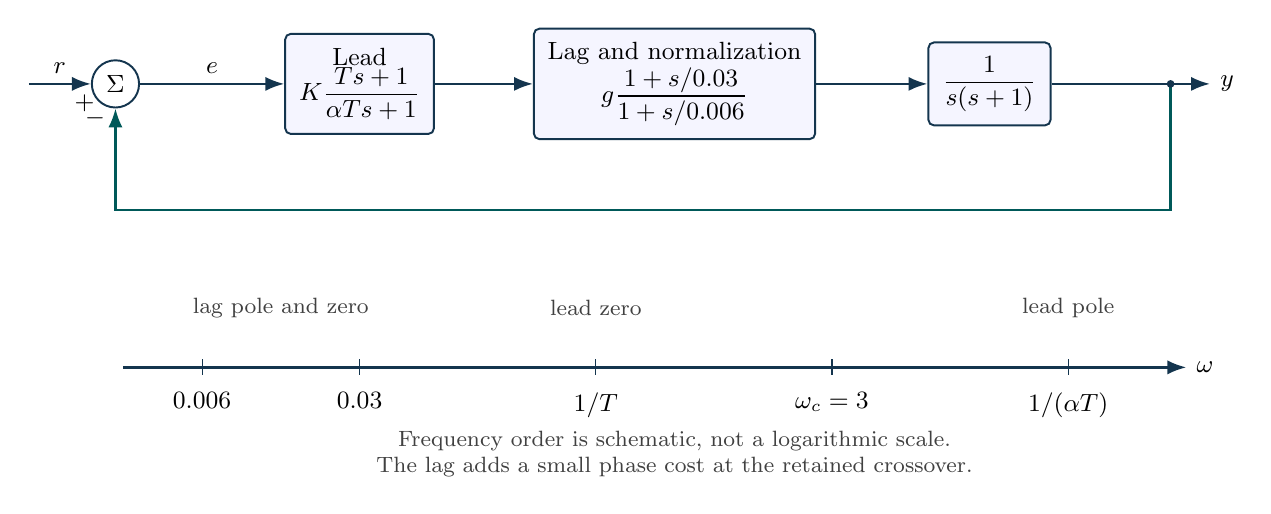
\begin{tikzpicture}[x=1cm,y=1cm,>=Latex,font=\small,
block/.style={draw=ink,fill=blue!4,rounded corners=2pt,minimum height=9mm,align=center,line width=.7pt,inner sep=5pt},
sum/.style={circle,draw=ink,fill=white,minimum size=6mm,inner sep=0pt,line width=.7pt},
sig/.style={->,draw=ink,line width=.85pt},
fb/.style={->,draw=teal!70!black,line width=.85pt},
dist/.style={->,draw=orange!75!black,line width=.85pt},
tap/.style={circle,fill=ink,inner sep=1.4pt},
note/.style={font=\footnotesize,align=center,text=black!75}]

\node[sum](e)at(.9,1.5){$\Sigma$};
\node[block](lead)at(4,1.5){Lead\\$K\dfrac{Ts+1}{\alpha Ts+1}$};
\node[block](lag)at(8,1.5){Lag and normalization\\$g\dfrac{1+s/0.03}{1+s/0.006}$};
\node[block](plant)at(12,1.5){$\dfrac{1}{s(s+1)}$};
\draw[sig](-.2,1.5)--node[above]{$r$}node[pos=.9,below]{$+$}(e);
\draw[sig](e)--node[above]{$e$}(lead);\draw[sig](lead)--(lag);\draw[sig](lag)--(plant);
\draw[sig](plant)--(14.8,1.5)node[right]{$y$};
\draw[fb](14.3,1.5)--(14.3,-.1)--(.9,-.1)--node[pos=.9,left]{$-$}(e);
\fill[ink](14.3,1.5)circle(1.4pt);
\draw[sig](1,-2.1)--(14.5,-2.1)node[right]{$\omega$};
\foreach \x/\lab in {2/0.006,4/0.03,7/{1/T},10/{\omega_c=3},13/{1/(\alpha T)}}{\draw[ink](\x,-2)--(\x,-2.2);\node[below=2mm]at(\x,-2.1){$\lab$};}
\node[note]at(3,-1.35){lag pole and zero};
\node[note]at(7,-1.35){lead zero};\node[note]at(13,-1.35){lead pole};
\node[note]at(8,-3.2){Frequency order is schematic, not a logarithmic scale.\\The lag adds a small phase cost at the retained crossover.};

\end{tikzpicture}
}\par{\small Lead and lag sections are drawn separately so their gain normalization and frequency ordering can be analyzed independently.}\end{center}
\begin{enumerate}
\item For the stable lead-compensated loop, calculate its velocity constant and unit-ramp error. State why the DC gain of G itself cannot be inserted as a finite number.
\answer The loop has one integrator, and $K_v=\lim_{s\to0}sC_{lead}G=C_{lead}(0)=K$. Thus $e_{ramp}=1/K\approx0.20942$. The plant has infinite DC gain because of its pole at zero, but the limit defining $K_v$ cancels that integrator and remains finite. The unit-step error is zero under nominal stable unity feedback. These steady errors do not specify transient overshoot.
\item Add $F(s)=(1+s/0.03)/(1+s/0.006)$ and multiply the controller by g so crossover remains at 3. Derive g, the new velocity constant and the new unit-ramp error.
\answer At 3 rad/s, $|F|=\sqrt{1+100^2}/\sqrt{1+500^2}$. Choose $g=1/|F|=\sqrt{250001/10001}\approx4.99976$. Because $F(0)=1$, the new velocity constant is $gK$, about 23.8739, and ramp error is $1/(gK)$, about 0.04189. Most of the low-frequency improvement comes from the renormalizing scalar gain. The explicit normalization convention must accompany any claim of a fivefold improvement.
\item Require unit-ramp error no greater than 0.05 and phase margin at least 55 degrees. Using the resulting design, check both requirements together rather than rounding the margin.
\answer The normalized lead--lag design has $K_v\simeq23.8739$ and ramp error about 0.041887, satisfying the 0.05 requirement. Its lag phase is negative, so the margin is approximately $54.54165^\circ$, below 55 degrees. Thus this exact design fails the combined specification even though tracking improves. Rounding the margin to 55 hides a violation; the lead phase, crossover or lag placement must be redesigned.
\end{enumerate}

\newpage
\task{4}{Spending the remaining phase reserve on a real communication link}
Evaluate the final lead--lag design after a pure communication delay is introduced. Keep strict stability and a desired robustness margin as separate requirements.
\begin{enumerate}
\item Compute the lag section phase at the retained crossover and the resulting phase margin. Explain why a lag network can improve low-frequency tracking while slightly reducing margin.
\answer At 3 rad/s the phase is $\arctan(100)-\arctan(500)\approx-0.45835^\circ$. Since the scalar renormalization has zero phase and crossover is retained, the new margin is $55-0.45835\approx54.54165^\circ$. The lag pole is closer to the origin than its zero, creating a band of negative phase. Placing both frequencies well below crossover limits that phase cost while permitting low-frequency gain improvement.
\item Assume the final lead-lag loop has the single crossover 3 rad/s and phase margin from Problem 4(a). Calculate its first constant-delay boundary and the delay allowance if at least 40 degrees of margin must remain. State the assumptions.
\answer A pure delay preserves magnitude and removes $3T_d$ radians at crossover. The first boundary is $T_{crit}=(54.54165\pi/180)/3\approx0.31731$ s. Retaining 40 degrees requires $T_d\le[(54.54165-40)\pi/180]/3\approx0.08460$ s. This uses the nominal stable loop, one relevant crossover and a constant pure delay. Sensor dynamics, uncertain plant gain or time-varying delays require re-evaluation.
\item A proposed link adds 0.09 s of constant pure delay. Does the model retain 40 degrees of margin? Is failure of that requirement equivalent to instability under the stated single-crossover assumptions?
\answer The remaining margin is $54.54165^\circ-3(0.09)180^\circ/\pi\simeq39.07179^\circ$, so the 40-degree requirement fails. However, 0.09 s is below the nominal first delay boundary of about 0.31731 s. Under the stated single-crossover pure-delay assumptions, the model remains stable while failing the stronger margin requirement. Neither conclusion covers arbitrary unmodeled poles, variable delay or actuator constraints.
\end{enumerate}

\newpage
\task{5}{A stable compensated output can still demand noisy actuator effort}
Check algebraic stability and then trace measurement noise to both physical output and controller output. These are different performance channels.
\begin{enumerate}
\item Derive the lead-only characteristic polynomial and use the cubic Routh inequality to check stability with the design formulas. Do not infer stability solely from an intended phase target.
\answer From $1+C_{lead}G=0$, the polynomial is $\alpha T s^3+(1+\alpha T)s^2+(1+KT)s+K$. All coefficients are positive. The remaining condition is $(1+\alpha T)(1+KT)>\alpha TK$. Expanding the left side minus the right gives $1+\alpha T+KT+\alpha KT^2-\alpha TK$, which can be evaluated with the actual designed parameters and is positive. The numerical root check in the validation script independently verifies negative real parts; arbitrary positive K,T,alpha should not be substituted without checking.
\item Let measurement be $y+n$ and feedback error be $r-y-n$. Derive the noise-to-output and noise-to-control transfers. Explain a high-frequency consequence of lead compensation.
\answer Solving $y=GC(r-y-n)$ gives $Y/N=-CG/(1+CG)=-T_c$, where $T_c$ is complementary sensitivity. Control satisfies $U/N=-C/(1+CG)=-CS$. At high frequency, plant gain tends to zero and $S\to1$, so control noise gain approaches $C(\infty)$. Lead-only $C(\infty)=K/\alpha$, larger than its DC gain K. Improved phase and bandwidth can therefore increase high-frequency actuator activity even when output noise remains small.
\item For the final controller $C=gK(Ts+1)(1+s/0.03)/[(\alpha Ts+1)(1+s/0.006)]$, find its high-frequency gain and the corresponding limiting noise-to-control and noise-to-output gains.
\answer The lead section tends to $K/\alpha$ and the lag section tends to $0.006/0.03=1/5$, so $C_\infty=gK/(5\alpha)$. Since $G(s)\sim1/s^2$, the loop tends to zero. Therefore $U/N=-C/(1+CG)\to-C_\infty$, whereas $Y/N=-CG/(1+CG)\to0$. A small high-frequency output response does not imply small actuator noise. This is an ideal high-frequency limit; a physical drive adds bandwidth and rate constraints.
\end{enumerate}

\end{document}
